\documentclass[
  doc,
  longtable,
  nolmodern,
  notxfonts,
  notimes,
  colorlinks=true,linkcolor=blue,citecolor=blue,urlcolor=blue]{apa7}

\usepackage{amsmath}
\usepackage{amssymb}

\geometry{inner=1in, outer=1in}
\fancyhfoffset[LE,RO]{0cm}



\RequirePackage{longtable}
\RequirePackage{threeparttablex}

\makeatletter
\renewcommand{\paragraph}{\@startsection{paragraph}{4}{\parindent}%
	{0\baselineskip \@plus 0.2ex \@minus 0.2ex}%
	{-.5em}%
	{\normalfont\normalsize\bfseries\typesectitle}}

\renewcommand{\subparagraph}[1]{\@startsection{subparagraph}{5}{0.5em}%
	{0\baselineskip \@plus 0.2ex \@minus 0.2ex}%
	{-\z@\relax}%
	{\normalfont\normalsize\bfseries\itshape\hspace{\parindent}{#1}\textit{\addperi}}{\relax}}
\makeatother




\usepackage{longtable, booktabs, multirow, multicol, colortbl, hhline, caption, array, float, xpatch}
\usepackage{subcaption}


\renewcommand\thesubfigure{\Alph{subfigure}}
\setcounter{topnumber}{2}
\setcounter{bottomnumber}{2}
\setcounter{totalnumber}{4}
\renewcommand{\topfraction}{0.85}
\renewcommand{\bottomfraction}{0.85}
\renewcommand{\textfraction}{0.15}
\renewcommand{\floatpagefraction}{0.7}

\usepackage{tcolorbox}
\tcbuselibrary{listings,theorems, breakable, skins}
\usepackage{fontawesome5}

\definecolor{quarto-callout-color}{HTML}{909090}
\definecolor{quarto-callout-note-color}{HTML}{0758E5}
\definecolor{quarto-callout-important-color}{HTML}{CC1914}
\definecolor{quarto-callout-warning-color}{HTML}{EB9113}
\definecolor{quarto-callout-tip-color}{HTML}{00A047}
\definecolor{quarto-callout-caution-color}{HTML}{FC5300}
\definecolor{quarto-callout-color-frame}{HTML}{ACACAC}
\definecolor{quarto-callout-note-color-frame}{HTML}{4582EC}
\definecolor{quarto-callout-important-color-frame}{HTML}{D9534F}
\definecolor{quarto-callout-warning-color-frame}{HTML}{F0AD4E}
\definecolor{quarto-callout-tip-color-frame}{HTML}{02B875}
\definecolor{quarto-callout-caution-color-frame}{HTML}{FD7E14}

%\newlength\Oldarrayrulewidth
%\newlength\Oldtabcolsep


\usepackage{hyperref}



\usepackage{color}
\usepackage{fancyvrb}
\newcommand{\VerbBar}{|}
\newcommand{\VERB}{\Verb[commandchars=\\\{\}]}
\DefineVerbatimEnvironment{Highlighting}{Verbatim}{commandchars=\\\{\}}
% Add ',fontsize=\small' for more characters per line
\usepackage{framed}
\definecolor{shadecolor}{RGB}{241,243,245}
\newenvironment{Shaded}{\begin{snugshade}}{\end{snugshade}}
\newcommand{\AlertTok}[1]{\textcolor[rgb]{0.68,0.00,0.00}{#1}}
\newcommand{\AnnotationTok}[1]{\textcolor[rgb]{0.37,0.37,0.37}{#1}}
\newcommand{\AttributeTok}[1]{\textcolor[rgb]{0.40,0.45,0.13}{#1}}
\newcommand{\BaseNTok}[1]{\textcolor[rgb]{0.68,0.00,0.00}{#1}}
\newcommand{\BuiltInTok}[1]{\textcolor[rgb]{0.00,0.23,0.31}{#1}}
\newcommand{\CharTok}[1]{\textcolor[rgb]{0.13,0.47,0.30}{#1}}
\newcommand{\CommentTok}[1]{\textcolor[rgb]{0.37,0.37,0.37}{#1}}
\newcommand{\CommentVarTok}[1]{\textcolor[rgb]{0.37,0.37,0.37}{\textit{#1}}}
\newcommand{\ConstantTok}[1]{\textcolor[rgb]{0.56,0.35,0.01}{#1}}
\newcommand{\ControlFlowTok}[1]{\textcolor[rgb]{0.00,0.23,0.31}{\textbf{#1}}}
\newcommand{\DataTypeTok}[1]{\textcolor[rgb]{0.68,0.00,0.00}{#1}}
\newcommand{\DecValTok}[1]{\textcolor[rgb]{0.68,0.00,0.00}{#1}}
\newcommand{\DocumentationTok}[1]{\textcolor[rgb]{0.37,0.37,0.37}{\textit{#1}}}
\newcommand{\ErrorTok}[1]{\textcolor[rgb]{0.68,0.00,0.00}{#1}}
\newcommand{\ExtensionTok}[1]{\textcolor[rgb]{0.00,0.23,0.31}{#1}}
\newcommand{\FloatTok}[1]{\textcolor[rgb]{0.68,0.00,0.00}{#1}}
\newcommand{\FunctionTok}[1]{\textcolor[rgb]{0.28,0.35,0.67}{#1}}
\newcommand{\ImportTok}[1]{\textcolor[rgb]{0.00,0.46,0.62}{#1}}
\newcommand{\InformationTok}[1]{\textcolor[rgb]{0.37,0.37,0.37}{#1}}
\newcommand{\KeywordTok}[1]{\textcolor[rgb]{0.00,0.23,0.31}{\textbf{#1}}}
\newcommand{\NormalTok}[1]{\textcolor[rgb]{0.00,0.23,0.31}{#1}}
\newcommand{\OperatorTok}[1]{\textcolor[rgb]{0.37,0.37,0.37}{#1}}
\newcommand{\OtherTok}[1]{\textcolor[rgb]{0.00,0.23,0.31}{#1}}
\newcommand{\PreprocessorTok}[1]{\textcolor[rgb]{0.68,0.00,0.00}{#1}}
\newcommand{\RegionMarkerTok}[1]{\textcolor[rgb]{0.00,0.23,0.31}{#1}}
\newcommand{\SpecialCharTok}[1]{\textcolor[rgb]{0.37,0.37,0.37}{#1}}
\newcommand{\SpecialStringTok}[1]{\textcolor[rgb]{0.13,0.47,0.30}{#1}}
\newcommand{\StringTok}[1]{\textcolor[rgb]{0.13,0.47,0.30}{#1}}
\newcommand{\VariableTok}[1]{\textcolor[rgb]{0.07,0.07,0.07}{#1}}
\newcommand{\VerbatimStringTok}[1]{\textcolor[rgb]{0.13,0.47,0.30}{#1}}
\newcommand{\WarningTok}[1]{\textcolor[rgb]{0.37,0.37,0.37}{\textit{#1}}}

\providecommand{\tightlist}{%
  \setlength{\itemsep}{0pt}\setlength{\parskip}{0pt}}
\usepackage{longtable,booktabs,array}
\usepackage{calc} % for calculating minipage widths
% Correct order of tables after \paragraph or \subparagraph
\usepackage{etoolbox}
\makeatletter
\patchcmd\longtable{\par}{\if@noskipsec\mbox{}\fi\par}{}{}
\makeatother
% Allow footnotes in longtable head/foot
\IfFileExists{footnotehyper.sty}{\usepackage{footnotehyper}}{\usepackage{footnote}}
\makesavenoteenv{longtable}

\usepackage{graphicx}
\makeatletter
\def\maxwidth{\ifdim\Gin@nat@width>\linewidth\linewidth\else\Gin@nat@width\fi}
\def\maxheight{\ifdim\Gin@nat@height>\textheight\textheight\else\Gin@nat@height\fi}
\makeatother
% Scale images if necessary, so that they will not overflow the page
% margins by default, and it is still possible to overwrite the defaults
% using explicit options in \includegraphics[width, height, ...]{}
\setkeys{Gin}{width=\maxwidth,height=\maxheight,keepaspectratio}
% Set default figure placement to htbp
\makeatletter
\def\fps@figure{htbp}
\makeatother


% definitions for citeproc citations
\NewDocumentCommand\citeproctext{}{}
\NewDocumentCommand\citeproc{mm}{%
  \begingroup\def\citeproctext{#2}\cite{#1}\endgroup}
\makeatletter
 % allow citations to break across lines
 \let\@cite@ofmt\@firstofone
 % avoid brackets around text for \cite:
 \def\@biblabel#1{}
 \def\@cite#1#2{{#1\if@tempswa , #2\fi}}
\makeatother
\newlength{\cslhangindent}
\setlength{\cslhangindent}{1.5em}
\newlength{\csllabelwidth}
\setlength{\csllabelwidth}{3em}
\newenvironment{CSLReferences}[2] % #1 hanging-indent, #2 entry-spacing
 {\begin{list}{}{%
  \setlength{\itemindent}{0pt}
  \setlength{\leftmargin}{0pt}
  \setlength{\parsep}{0pt}
  % turn on hanging indent if param 1 is 1
  \ifodd #1
   \setlength{\leftmargin}{\cslhangindent}
   \setlength{\itemindent}{-1\cslhangindent}
  \fi
  % set entry spacing
  \setlength{\itemsep}{#2\baselineskip}}}
 {\end{list}}
\usepackage{calc}
\newcommand{\CSLBlock}[1]{\hfill\break\parbox[t]{\linewidth}{\strut\ignorespaces#1\strut}}
\newcommand{\CSLLeftMargin}[1]{\parbox[t]{\csllabelwidth}{\strut#1\strut}}
\newcommand{\CSLRightInline}[1]{\parbox[t]{\linewidth - \csllabelwidth}{\strut#1\strut}}
\newcommand{\CSLIndent}[1]{\hspace{\cslhangindent}#1}





\usepackage{newtx}

\defaultfontfeatures{Scale=MatchLowercase}
\defaultfontfeatures[\rmfamily]{Ligatures=TeX,Scale=1}





\title{Hypothesis Testing Using Bayes Factor in Behavioral Sciences}


\shorttitle{Test Bayes Factor}


\usepackage{etoolbox}









\authorsnames[{1},{2}]{Timo B. Roettger,Michael Franke}







\authorsaffiliations{
{Department of Linguistics \& Scandinavian Studies, University of
Oslo},{Department of Linguistics, University of Tübingen}}




\leftheader{Roettger and Franke}



\abstract{Recent times have seen a surge of Bayesian inference across
the behavioral sciences. However, the process of testing hypothesis is
often conceptually challenging or computationally costly. This tutorial
provides an accessible, non-technical introduction that covers the most
common scenarios in experimental sciences: Testing the evidence for an
alternative hypothesis using Bayes Factor through the Savage Dickey
approximation. This method is conceptually easy to understand and
computatioanlly cheap. }

\keywords{statistics, Bayes, Bayes Factor, Savage Dickey, hypothesis
testing, ROPE}

\authornote{\par{\addORCIDlink{Timo B. Roettger}{0000-0003-1400-2739}} 
\par{ }
\par{   The authors have no conflict of interest to declare.    }
\par{Correspondence concerning this article should be addressed to Timo
B.
Roettger, Email: \href{mailto:timo.roettger@iln.uio.no}{timo.roettger@iln.uio.no}}
}

\makeatletter
\let\endoldlt\endlongtable
\def\endlongtable{
\hline
\endoldlt
}
\makeatother

\urlstyle{same}



\makeatletter
\@ifpackageloaded{caption}{}{\usepackage{caption}}
\AtBeginDocument{%
\ifdefined\contentsname
  \renewcommand*\contentsname{Table of contents}
\else
  \newcommand\contentsname{Table of contents}
\fi
\ifdefined\listfigurename
  \renewcommand*\listfigurename{List of Figures}
\else
  \newcommand\listfigurename{List of Figures}
\fi
\ifdefined\listtablename
  \renewcommand*\listtablename{List of Tables}
\else
  \newcommand\listtablename{List of Tables}
\fi
\ifdefined\figurename
  \renewcommand*\figurename{Figure}
\else
  \newcommand\figurename{Figure}
\fi
\ifdefined\tablename
  \renewcommand*\tablename{Table}
\else
  \newcommand\tablename{Table}
\fi
}
\@ifpackageloaded{float}{}{\usepackage{float}}
\floatstyle{ruled}
\@ifundefined{c@chapter}{\newfloat{codelisting}{h}{lop}}{\newfloat{codelisting}{h}{lop}[chapter]}
\floatname{codelisting}{Listing}
\newcommand*\listoflistings{\listof{codelisting}{List of Listings}}
\makeatother
\makeatletter
\makeatother
\makeatletter
\@ifpackageloaded{caption}{}{\usepackage{caption}}
\@ifpackageloaded{subcaption}{}{\usepackage{subcaption}}
\makeatother

% From https://tex.stackexchange.com/a/645996/211326
%%% apa7 doesn't want to add appendix section titles in the toc
%%% let's make it do it
\makeatletter
\xpatchcmd{\appendix}
  {\par}
  {\addcontentsline{toc}{section}{\@currentlabelname}\par}
  {}{}
\makeatother

%% Disable longtable counter
%% https://tex.stackexchange.com/a/248395/211326

\usepackage{etoolbox}

\makeatletter
\patchcmd{\LT@caption}
  {\bgroup}
  {\bgroup\global\LTpatch@captiontrue}
  {}{}
\patchcmd{\longtable}
  {\par}
  {\par\global\LTpatch@captionfalse}
  {}{}
\apptocmd{\endlongtable}
  {\ifLTpatch@caption\else\addtocounter{table}{-1}\fi}
  {}{}
\newif\ifLTpatch@caption
\makeatother

\begin{document}

\maketitle



\setcounter{secnumdepth}{3}

\setlength\LTleft{0pt}




\section{Introduction}\label{introduction}

To date, the most common quantitative approach across the experimental
sciences is to run an experiment with one or more predictors and
statistically test whether the predictors affect the measured variables.
Traditionally, these statistical tests have been done within the null
hypothesis significance testing framework. Over the last decade or so,
however, we have seen more and more statistical approaches within an
alternative inferential framework: Bayesian inference. Testing
hypothesis within the Bayesian framework is often considered either
conceptually challenging, computationally too costly, or both. This
tutorial provides an accessible, non-technical introduction to Bayesian
hypothesis testing that is easy to understand and computationally cheap.

\section{Motivation and intended
audience}\label{motivation-and-intended-audience}

This tutorial provides a very basic introduction to the topic using R (R
Core Team, 2025). We wrote this tutorial with a particular reader in
mind. If you have used R before and if you have a basic understanding of
linear regression, and Bayesian inference, this tutorial is for you. We
will remain mostly conceptual to provide you with a conceptual tool to
approach hypothesis testing within Bayesian inference. The form of
hypothesis testing that we would like to introduce to you is, however,
different from the traditional null hypothesis significance testing in
that it requires more thinking about the quantitative nature of your
data. This is not a bug but, at least for us, a feature that will allow
you to understand both your data and what you can learn from them
better.

If you don't have any experience with regression modeling, you will
probably still be able to follow, but you might also want to consider
doing a crash course. To bring you up to speed, we recommend the
excellent tutorial by Bodo Winter
(\citeproc{ref-winter_Linear_preprint_2013}{2013}) on mixed effects
regression in a non-Bayesian ---a.k.a. frequentist---paradigm. To then
make the transition to Bayesian versions of these regression models, we
shamelessly suggest our own tutorial on ``Bayesian Regression for
Factorial Designs'' as a natural follow-up using the same data and
Winter (\citeproc{ref-franke-roettger_Bayesian_preprint_2019}{Franke \&
Roettger, 2019}). In a sense, the present tutorial on hypothesis testing
could be considered the long-awaited sequel of the series started by
Winter. For continuity, we will continue to use the original data set.

To actively follow this tutorial, you should have R installed on your
computer (https://www.r-project.org). Unless you already have a favorite
editor for tinkering with R scripts, we recommend to try out RStudio
(https://www.rstudio.com). You will also need some packages, which you
can import with the following code:

\begin{Shaded}
\begin{Highlighting}[]
\CommentTok{\# package for convenience functions (e.g. plotting)}
\FunctionTok{library}\NormalTok{(tidyverse)}
\FunctionTok{library}\NormalTok{(ggdist)}

\CommentTok{\# package for Bayesian regression modeling}
\FunctionTok{library}\NormalTok{(brms)}

\CommentTok{\# package for posterior wrangling and plotting}
\FunctionTok{library}\NormalTok{(tidybayes)}

\CommentTok{\# package for BF calculation and plotting}
\FunctionTok{library}\NormalTok{(bayestestR)}
\end{Highlighting}
\end{Shaded}

\section{Data, research questions \&
hypotheses}\label{data-research-questions-hypotheses}

This tutorial looks at a data set relevant for investigating whether
voice pitch differs across social contexts in Korean. Korean is a
language in which the social distance between speakers plays a central
role. The way Korean speakers speak depends for example on whether they
are in a formal context (e.g.~during a consultation with a professor) or
an informal context (e.g.~chatting with a friend about the holidays)
(\citeproc{ref-winter-grawunder_Phonetic_journalarticle_2012}{Winter \&
Grawunder, 2012}).

To load the data into your R environment, run the following code

\begin{Shaded}
\begin{Highlighting}[]
\CommentTok{\# TO DO: STORE ONLINE}
\CommentTok{\# TO DO: SIMPLIFY STORED DATA}
\NormalTok{polite }\OtherTok{=} \FunctionTok{read\_csv}\NormalTok{(}\StringTok{"../data/polite.csv"}\NormalTok{) }\SpecialCharTok{|\textgreater{}} 
  \CommentTok{\# remove men}
  \FunctionTok{filter}\NormalTok{(gender }\SpecialCharTok{==} \StringTok{"F"}\NormalTok{) }\SpecialCharTok{|\textgreater{}} 
  \CommentTok{\# calculate semitones (reference 50 Hz)}
  \FunctionTok{mutate}\NormalTok{(}\AttributeTok{pitch\_ST =} \DecValTok{12} \SpecialCharTok{*} \FunctionTok{log2}\NormalTok{(pitch }\SpecialCharTok{/} \DecValTok{50}\NormalTok{))}

\NormalTok{polite}
\end{Highlighting}
\end{Shaded}

\begin{verbatim}
# A tibble: 126 x 5
   subject gender context  pitch pitch_ST
   <chr>   <chr>  <chr>    <dbl>    <dbl>
 1 F1      F      formal    215.     25.2
 2 F1      F      informal  211.     24.9
 3 F1      F      formal    285.     30.1
 4 F1      F      informal  266.     28.9
 5 F1      F      formal    211.     24.9
 6 F1      F      informal  286.     30.2
 7 F1      F      formal    252.     28.0
 8 F1      F      informal  282.     29.9
 9 F1      F      formal    230.     26.4
10 F1      F      informal  250.     27.9
# i 116 more rows
\end{verbatim}

This data set contains anonymous identifiers for individual speakers
stored in the variable \texttt{subject.} In this tutorial we will only
be looking at female speakers btw. Subjects produced different sentences,
and the experiment manipulated whether the sentences were produced in a
\texttt{formal} or an \texttt{informal} social context, indicated by the
variable \texttt{context.} Crucially, each row contains a measurement of
pitch in Hz stored in the variable \texttt{pitch}. Here we have
calculated a derived scale (semitones) of pitch which more closely
resembles the way people perceive pitch (\texttt{pitch\_ST})

For most analyses of behavioral experiments, researchers are interested
in whether an outcome variable is meaningfully affected by at least one
manipulated variable and if so how the outcome variable is affected by
it. In this case, Winter and Grawunder
(\citeproc{ref-winter-grawunder_Phonetic_journalarticle_2012}{2012})
wanted to test whether pitch is meaningfully affected by the social
context of the utterance.

As a first step, we can explore this question visually:

\begin{figure}[H]

\caption{Empirical distribution of pitch values across contexts}

{\centering 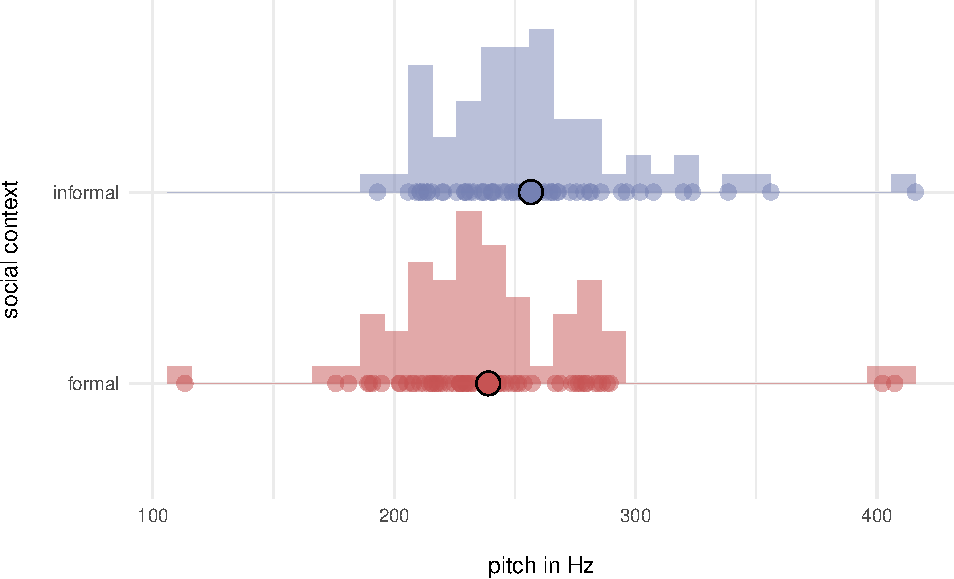
\includegraphics{manuscript_files/figure-pdf/descriptive-dataviz-1.pdf}

}

\end{figure}%

Figure 1 displays the pitch values for all utterances in the dataset
across contexts (semi-transparent points). The solid points indicate the
average pitch values across all sentences and speakers. Looking at the
plot, we can see that voice pitch from utterances in formal contexts are
on average slightly lower than those in informal contexts. The red
distribution is slightly shifted to the left of the blue distribution by
around 1.3 semitones. In other words, speakers tend to slightly lower
their voice pitch when speaking in a formal context. But there is also a
lot of overlap between the two contexts. Now as Bayesians, we would like
to translate the data into an expression of evidence: does the data
provide evidence for our research hypotheses?

Let us build a Bayesian linear model to approach an answer to this
question. Our first step is to specify the model formula and check which
priors need to be specified:

\begin{Shaded}
\begin{Highlighting}[]
\CommentTok{\# define linear model formula}
\CommentTok{\# predict pitch by context and allow for that relationship }
\CommentTok{\# to vary between subjects}
\NormalTok{formula }\OtherTok{\textless{}{-}} \FunctionTok{bf}\NormalTok{(pitch\_ST }\SpecialCharTok{\textasciitilde{}}\NormalTok{ context }\SpecialCharTok{+}\NormalTok{ (}\DecValTok{1} \SpecialCharTok{+}\NormalTok{ context }\SpecialCharTok{|}\NormalTok{ subject))}

\CommentTok{\# get priors for this model}
\FunctionTok{get\_prior}\NormalTok{(formula, polite)}
\end{Highlighting}
\end{Shaded}

The default priors that brms picks for the Intercept and the variance
parameters are mostly reasonable as they are derived from the data,
weakly informative and symmetrical. However the prior for our critical
parameter \texttt{contextinformal} should also be weakly informative
(\citeproc{ref-gelman-etal_Prior_journalarticle_2017}{Gelman et al.,
2017}), i.e.~the prior assumption about the difference between informal
and formal contexts should be that we don't know, but our best guess is
that it is close to zero and equally likely to be more or less than
zero. So we specify a normal distribution centered on zero for this
parameter.

Note: Only for demonstration purposes, we will use default priors for
the other parameters. You always should critically reflect on all of
your priors.

\begin{Shaded}
\begin{Highlighting}[]
\CommentTok{\# }\AlertTok{NOTE}\CommentTok{: TO MAKE IT EASIER TO FOLLOW WE COULD CONTRAST CODE THE PREDICTOR}

\CommentTok{\# pick a weakly informative prior for the critical parameter}
\NormalTok{priors }\OtherTok{\textless{}{-}} \FunctionTok{prior}\NormalTok{(}\FunctionTok{normal}\NormalTok{(}\DecValTok{0}\NormalTok{, }\DecValTok{2}\NormalTok{), }
                \AttributeTok{class =}\NormalTok{ b, }
                \AttributeTok{coef =} \StringTok{"contextinformal"}\NormalTok{)}
\end{Highlighting}
\end{Shaded}

Now we do a so-called prior predictive check, in other words we want to
know what the posterior distribution looks like before having seen the
data, based on the priors only. This is a useful exercise to make sure
that the priors results in reasonable quantitative assumptions. We
usually do it for all parameters, but here we will focus only on the
critical parameter \texttt{contextinformal}, i.e.~the difference between
formal and informal contexts. Let us also have a look at the predictions
for the prior-only model.

\begin{Shaded}
\begin{Highlighting}[]
\CommentTok{\# }\AlertTok{NOTE}\CommentTok{: CAN WE STORE THE SAMPLING PARAMETERS (seed, iter, chains, cores, backend, data)? }
\CommentTok{\#       TO MAKE THE CODE CHUNKS SMALLER?}

\CommentTok{\# run the model}
\NormalTok{fit\_prior }\OtherTok{\textless{}{-}} \FunctionTok{brm}\NormalTok{(formula,}
           \AttributeTok{prior =}\NormalTok{ priors,}
           \AttributeTok{family =} \FunctionTok{gaussian}\NormalTok{(),}
           \CommentTok{\# sample prior only}
           \AttributeTok{sample\_prior =} \StringTok{"only"}\NormalTok{,}
           \CommentTok{\# common sampling specifications}
           \AttributeTok{file  =} \StringTok{"../models/fit\_prior"}\NormalTok{,}
           \AttributeTok{seed =} \DecValTok{1234}\NormalTok{,}
           \AttributeTok{iter =} \DecValTok{8000}\NormalTok{,}
           \AttributeTok{chains =} \DecValTok{4}\NormalTok{,}
           \AttributeTok{cores =} \DecValTok{4}\NormalTok{,}
           \AttributeTok{backend =} \StringTok{"cmdstanr"}\NormalTok{,}
           \AttributeTok{data =}\NormalTok{ polite)}
\end{Highlighting}
\end{Shaded}

\begin{Shaded}
\begin{Highlighting}[]
\CommentTok{\# extract prior samples}
\NormalTok{prior\_samples }\OtherTok{\textless{}{-}} 
\NormalTok{  fit\_prior }\SpecialCharTok{|\textgreater{}} 
  \FunctionTok{spread\_draws}\NormalTok{(b\_contextinformal)}
  
\CommentTok{\# plot  }
\FunctionTok{ggplot}\NormalTok{(prior\_samples,}
       \FunctionTok{aes}\NormalTok{(}\AttributeTok{x =}\NormalTok{ b\_contextinformal)) }\SpecialCharTok{+} 
  \FunctionTok{stat\_histinterval}\NormalTok{(}\AttributeTok{slab\_color =}\NormalTok{ project\_colors[}\DecValTok{11}\NormalTok{],}
                    \AttributeTok{slab\_fill =} \FunctionTok{alpha}\NormalTok{(project\_colors[}\DecValTok{11}\NormalTok{], }\FloatTok{0.5}\NormalTok{),}
                    \AttributeTok{fill =} \ConstantTok{NA}\NormalTok{,}
                    \AttributeTok{color =} \ConstantTok{NA}\NormalTok{,}
                    \AttributeTok{outline\_bars =} \ConstantTok{FALSE}\NormalTok{) }\SpecialCharTok{+}
  \FunctionTok{labs}\NormalTok{(}\AttributeTok{x =} \StringTok{"}\SpecialCharTok{\textbackslash{}n}\StringTok{ pitch difference in semitones"}\NormalTok{,}
       \AttributeTok{y =} \StringTok{"density }\SpecialCharTok{\textbackslash{}n}\StringTok{"}\NormalTok{) }\SpecialCharTok{+}
  \FunctionTok{scale\_x\_continuous}\NormalTok{(}\AttributeTok{limits =}\FunctionTok{c}\NormalTok{(}\SpecialCharTok{{-}}\DecValTok{4}\NormalTok{,}\DecValTok{4}\NormalTok{)) }\SpecialCharTok{+}
  \FunctionTok{theme\_minimal}\NormalTok{() }
\end{Highlighting}
\end{Shaded}

\begin{figure}[H]

\caption{Prior probability of the effect of context on pitch,
i.e.~before seeing the data}

{\centering 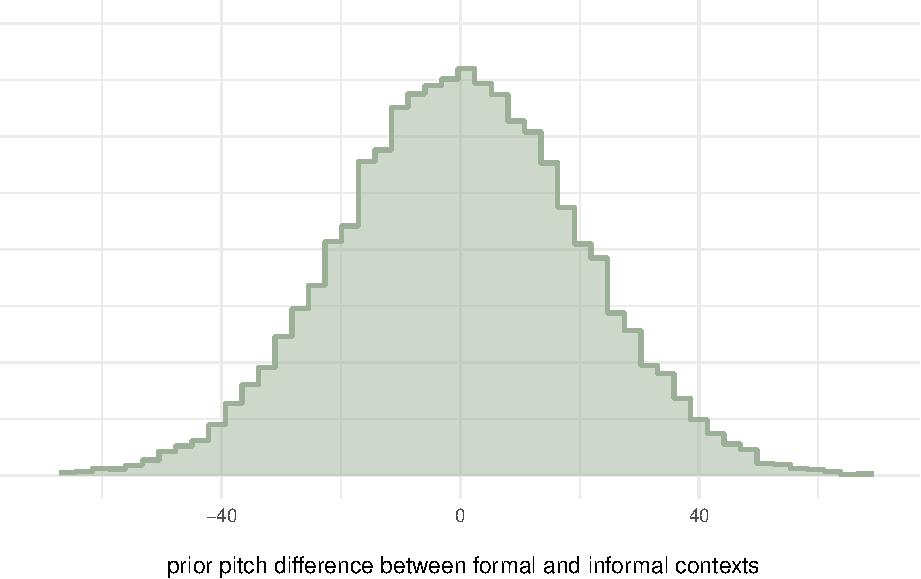
\includegraphics{manuscript_files/figure-pdf/plot-priors-1.pdf}

}

\end{figure}%

Looking at the distribution, the priors for the effect of context on
pitch seems sensible. The most plausible value is zero. Values that are
smaller or larger than zero become less plausible the further they are
away from zero and values being smaller or larger than zero are equally
likely. Good. Before we have seen the data, our model is somewhat
pessimistic about the effect of context on on pitch. Now we can run the
full model that integrates the likelihood (our data) with the priors and
visualize the posteriors for the critical parameter.

\begin{Shaded}
\begin{Highlighting}[]
\CommentTok{\# run the model}
\NormalTok{fit }\OtherTok{\textless{}{-}} \FunctionTok{brm}\NormalTok{(formula,}
           \AttributeTok{prior =}\NormalTok{ priors,}
           \AttributeTok{family =} \FunctionTok{gaussian}\NormalTok{(),}
           \CommentTok{\# common sampling specifications}
           \AttributeTok{file  =} \StringTok{"../models/fit"}\NormalTok{,}
           \AttributeTok{seed =} \DecValTok{1234}\NormalTok{,}
           \AttributeTok{iter =} \DecValTok{4000}\NormalTok{,}
           \AttributeTok{chains =} \DecValTok{4}\NormalTok{,}
           \AttributeTok{cores =} \DecValTok{4}\NormalTok{,}
           \AttributeTok{backend =} \StringTok{"cmdstanr"}\NormalTok{,}
           \AttributeTok{data =}\NormalTok{ polite)}
\end{Highlighting}
\end{Shaded}

\begin{Shaded}
\begin{Highlighting}[]
\NormalTok{posterior\_plot }\OtherTok{\textless{}{-}} 
\NormalTok{  fit }\SpecialCharTok{|\textgreater{}} 
  \FunctionTok{spread\_draws}\NormalTok{(b\_contextinformal) }\SpecialCharTok{|\textgreater{}} 
  \FunctionTok{ggplot}\NormalTok{(}\FunctionTok{aes}\NormalTok{(}\AttributeTok{x =}\NormalTok{ b\_contextinformal)) }\SpecialCharTok{+} 
    \FunctionTok{stat\_histinterval}\NormalTok{(}\AttributeTok{data =}\NormalTok{ prior\_samples,}
                     \AttributeTok{slab\_color =}\NormalTok{ project\_colors[}\DecValTok{11}\NormalTok{],}
                     \AttributeTok{slab\_fill =} \FunctionTok{alpha}\NormalTok{(project\_colors[}\DecValTok{11}\NormalTok{], }\FloatTok{0.5}\NormalTok{),}
                     \AttributeTok{fill =} \ConstantTok{NA}\NormalTok{,}
                     \AttributeTok{color =} \ConstantTok{NA}\NormalTok{,}
                     \AttributeTok{outline\_bars =} \ConstantTok{FALSE}\NormalTok{) }\SpecialCharTok{+}
    \FunctionTok{stat\_histinterval}\NormalTok{(}\AttributeTok{slab\_color =}\NormalTok{ project\_colors[}\DecValTok{14}\NormalTok{],}
                      \AttributeTok{slab\_fill =} \FunctionTok{alpha}\NormalTok{(project\_colors[}\DecValTok{14}\NormalTok{], }\FloatTok{0.5}\NormalTok{),}
                      \AttributeTok{color =} \ConstantTok{NA}\NormalTok{,}
                      \AttributeTok{outline\_bars =} \ConstantTok{FALSE}\NormalTok{) }\SpecialCharTok{+}
  \CommentTok{\# stat\_slab(data = prior\_samples,}
  \CommentTok{\#           lwd = 1,}
  \CommentTok{\#           colour = project\_colors[11],}
  \CommentTok{\#           fill = NA) +}
  \FunctionTok{scale\_thickness\_shared}\NormalTok{() }\SpecialCharTok{+}
  \FunctionTok{scale\_x\_continuous}\NormalTok{(}\AttributeTok{limits =}\FunctionTok{c}\NormalTok{(}\SpecialCharTok{{-}}\DecValTok{4}\NormalTok{,}\DecValTok{4}\NormalTok{)) }\SpecialCharTok{+}
  \FunctionTok{labs}\NormalTok{(}\AttributeTok{x =} \StringTok{"}\SpecialCharTok{\textbackslash{}n}\StringTok{ pitch difference in semitones"}\NormalTok{,}
       \AttributeTok{y =} \StringTok{"density }\SpecialCharTok{\textbackslash{}n}\StringTok{"}\NormalTok{) }\SpecialCharTok{+}
  \FunctionTok{theme\_minimal}\NormalTok{() }\SpecialCharTok{+}
  \FunctionTok{theme}\NormalTok{(}\AttributeTok{legend.position =} \StringTok{"top"}\NormalTok{)}

\NormalTok{posterior\_plot}
\end{Highlighting}
\end{Shaded}

\begin{figure}[H]

\caption{Posterior probability of the effect of context on pitch,
i.e.~after seeing the data}

{\centering 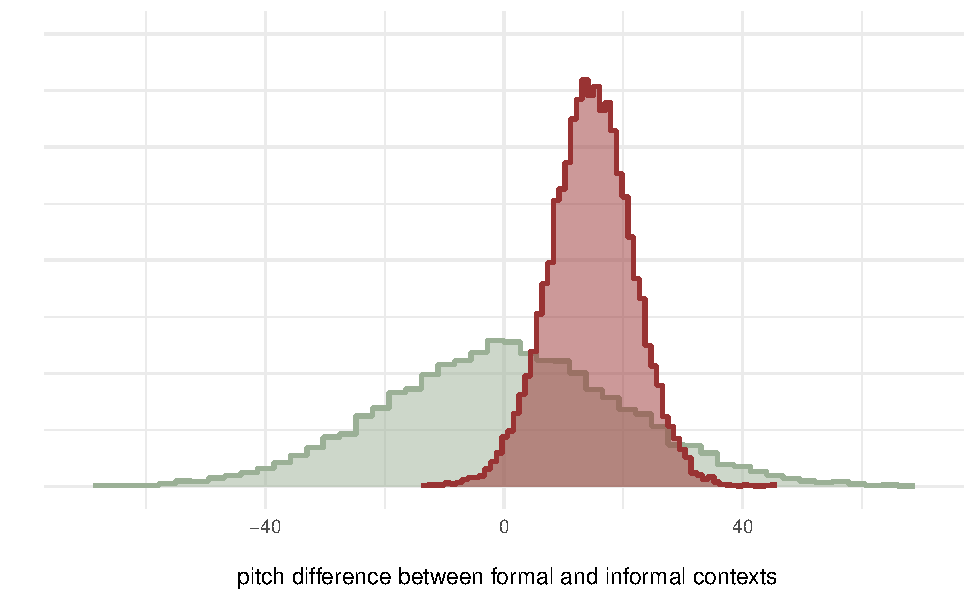
\includegraphics{manuscript_files/figure-pdf/plot-posterior-1.pdf}

}

\end{figure}%

The posterior samples suggests that the majority of plausible values
after seeing the data are positive, or in other words, informal contexts
elicit larger pitch values. Negative values are not very plausible
values, but also not completely implausible. Compared to our prior
probability (green distribution) for which roughly 50\% of posteriors
were negative, this decrease in plausibility of negative values is quite
noteworthy already.

What we have done here should be quite familiar. We compare our model
predictions to a reference point. It is a single point value: zero.But
do we really care that much for such point hypotheses? Is zero really
that special? We might think so because years of using null hypothesis
significance testing has conditioned us to think that way. But this
tutorial would like to break this cycle and move forward. Bear with us
and let's approach hypothesis testing a bit differently today.

\subsection{Grounding hypotheses in regions of practical
equivalences}\label{grounding-hypotheses-in-regions-of-practical-equivalences}

NOTE NEED TO FIND A BETTER JND SOURCE

Above we claimed that we wanted to test ``whether pitch is
\textbf{meaningfully affected} by the social context of the utterance''.
We snuck the word meaningfully in there for a reason. But what does
``meaningful'' mean? This is really a good questions and (un)fortunately
requires quite a bit of thinking. This tutorial deals with speech data.
Speech is, in spoken languages at least, THE vehicle to transmit
linguistic information in order to communicate with each other. Speech
is also very complex and very noisy: Not everything that can be measured
in the acoustic signal matters for the listener. For example, if
something cannot be perceived reliably, it is at least conceivable that
it might play little to no role in communication. While speech sciences
has a rich research tradition to estimate what can and what cannot be
reliably heard, exact estimates depends on a lot of moving parts. But
there is evidence that pitch in static conditions with resynthesised
speech might be around 5\%
(\citeproc{ref-isacenko-schadlich_Model_book_1970}{Isačenko \&
Schädlich, 1970}). That means, pitch changes below 0.05 semitones can
not be used to discriminate two sounds reliably. Such thresholds are
referred to as Just Noticeable Differences (JNDs) and can be used to
define what constitutes meaningful differences when we look at speech
data. So we could interpret the original hypothesis the following way:
If a pitch difference is below the JND, it is not meaningful. So instead
of testing against a point-zero hypothesis, we can test against a range
of parameter values that are equivalent to the null value for practical
purposes. In our case, let us be extra conservative and double the
reported JND to 0.1, so values between \texttt{-0.1} and \texttt{0.1}
are simply meaningless. Such ranges are sometimes called regions of
practical equivalence (ROPEs). Alternative terms that have been used are
range of equivalence, equivalence margin, smallest effect size of
interest, and good-enough belt (see
\citeproc{ref-kruschke_Rejecting_journalarticle_2018}{Kruschke, 2018}).

\begin{Shaded}
\begin{Highlighting}[]
\NormalTok{rope }\OtherTok{\textless{}{-}} \FunctionTok{c}\NormalTok{(}\SpecialCharTok{{-}}\FloatTok{0.1}\NormalTok{,}\FloatTok{0.1}\NormalTok{)}
\end{Highlighting}
\end{Shaded}

With a ROPE being defined, we can now test our hypothesis ``whether
pitch is \textbf{meaningfully affected} by the social context of the
utterance'' using Bayes Factor:

\section{Testing hypothesis using Bayes
Factor}\label{testing-hypothesis-using-bayes-factor}

\subsection{What is Bayes Factor}\label{what-is-bayes-factor}

Bayes Factors (henceforth: BFs) allow us to quantify relative evidence
of one model compared to another.

\subsection{Approximating Bayes Factor with Savage
Dickey}\label{approximating-bayes-factor-with-savage-dickey}

\subsection{Calculating Bayes Factor for a specified Region of Practical
Equivalence
(ROPE)}\label{calculating-bayes-factor-for-a-specified-region-of-practical-equivalence-rope}

Instead of doing it by hand, we can calculate the Savage Dickey ratio
with the \texttt{bayesfactor\_parameters()} function from the
\texttt{bayesfactorR} package. What happens behind the scenes is that
the function will sample posteriors from your specified model based on
priors only (so before seeing any data) and calculates the posterior
probability of the specified \texttt{null} hypothesis (here the range
specified by our ROPE).

\begin{Shaded}
\begin{Highlighting}[]
\CommentTok{\#|warning: FALSE}
\CommentTok{\#|message: FALSE}

\NormalTok{BF\_1 }\OtherTok{\textless{}{-}} \FunctionTok{bayesfactor\_parameters}\NormalTok{(}\AttributeTok{posterior =}\NormalTok{ fit, }
                               \AttributeTok{null =}\NormalTok{ rope, }
                               \AttributeTok{parameter =} \StringTok{"b\_contextinformal"}\NormalTok{)}
\end{Highlighting}
\end{Shaded}

Before interpreting the number we get, let us visually explore what our
BF corresponds to.

\begin{Shaded}
\begin{Highlighting}[]
\NormalTok{posterior\_plot }\SpecialCharTok{+} 
  \FunctionTok{geom\_vline}\NormalTok{(}\AttributeTok{xintercept =} \FunctionTok{c}\NormalTok{(rope[}\DecValTok{1}\NormalTok{], rope[}\DecValTok{2}\NormalTok{]),}
             \AttributeTok{lty =} \StringTok{"dashed"}\NormalTok{)}
\end{Highlighting}
\end{Shaded}

\begin{figure}[H]

\caption{Prior and posterior probability of the effect of context on
pitch relative to the ROPE (-0.1, 0.1)}

{\centering 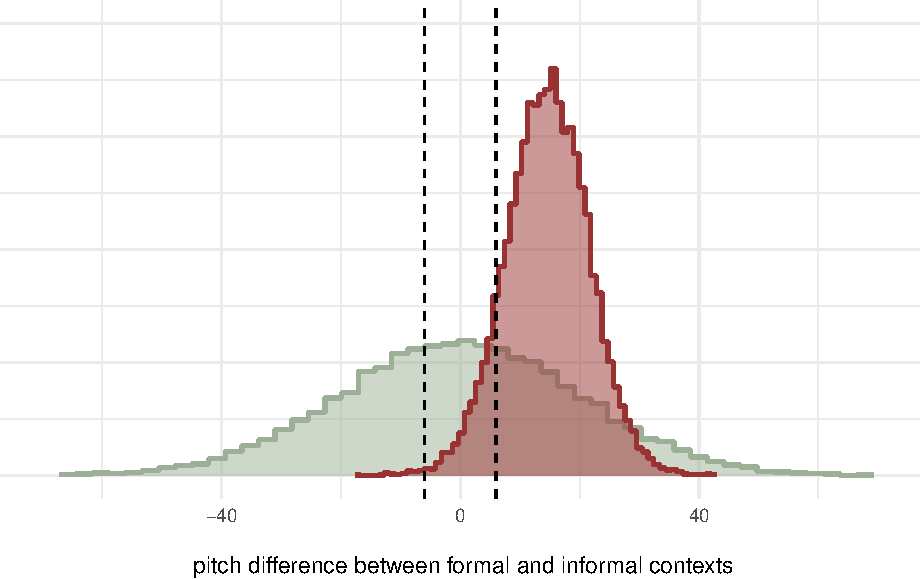
\includegraphics{manuscript_files/figure-pdf/plot-ropes-1.pdf}

}

\end{figure}%

What the BF does is relating two numbers: (a) The prior probability of
parameter values outside the rope, i.e.~the proportion of the green
distribution that falls outside the dashed lines, and (b) the posterior
probability of parameter values outside the rope, i.e.~the proportion of
the red distribution that falls outside the dashed lines. Eye-balling
the plot, we can maybe already see that more of the red distribution is
outside the ROPE than of the green distribution.

\begin{Shaded}
\begin{Highlighting}[]
\NormalTok{BF\_1}
\end{Highlighting}
\end{Shaded}

\begin{verbatim}
Bayes Factor (Null-Interval)

Parameter       |   BF
----------------------
contextinformal | 5.76

* Evidence Against The Null: [-0.100, 0.100]
\end{verbatim}

To be exact, 5.6 times for of the red distribution is outside the ROPE
than of the green distribution.

That means the model that has seen the data provide 5.6 times more
evidence for pitch being outside of the ROPE, or in other words, it is
5.6 times more likely (after having seen the data), that context affects
pitch meaningfully. According to Lee and Wagenmakers
(\citeproc{ref-lee-wagenmakers_Bayesian_book_2014}{2014}) criteria for
interpreting BFs, this value corresponds to moderate evidence for the
alternative hypothesis.

\subsection{Sensitivity analysis for different priors and
ROPEs}\label{sensitivity-analysis-for-different-priors-and-ropes}

Now as you probably have guessed already, all these probabilities are
very much dependent on the priors of the model, so it is important to
evaluate the robustness of our BF-based interpretation across a range of
sensible priors. And as long as we are not a 100\% sure about our ROPEs,
we might as well explore the robustness of the BF across different
ROPEs. We won't bore you with the code for that process, but you can
follow it along in our scripts. Let us assume the following five ROPE
intervals centered on zero: 0.05, 0.1, 0.5, 1, 2. We assume the
following five prior values for the width of the standard deviation of
the critical parameter (centered on zero): 1 1.5, 2, 2.5, 3. These are
all sensible prior widths assuming that medium to strong effects in
either direction are plausible.

\begin{figure}[H]

\caption{Bayes Factors for a range of priors and a range of ROPEs}

{\centering 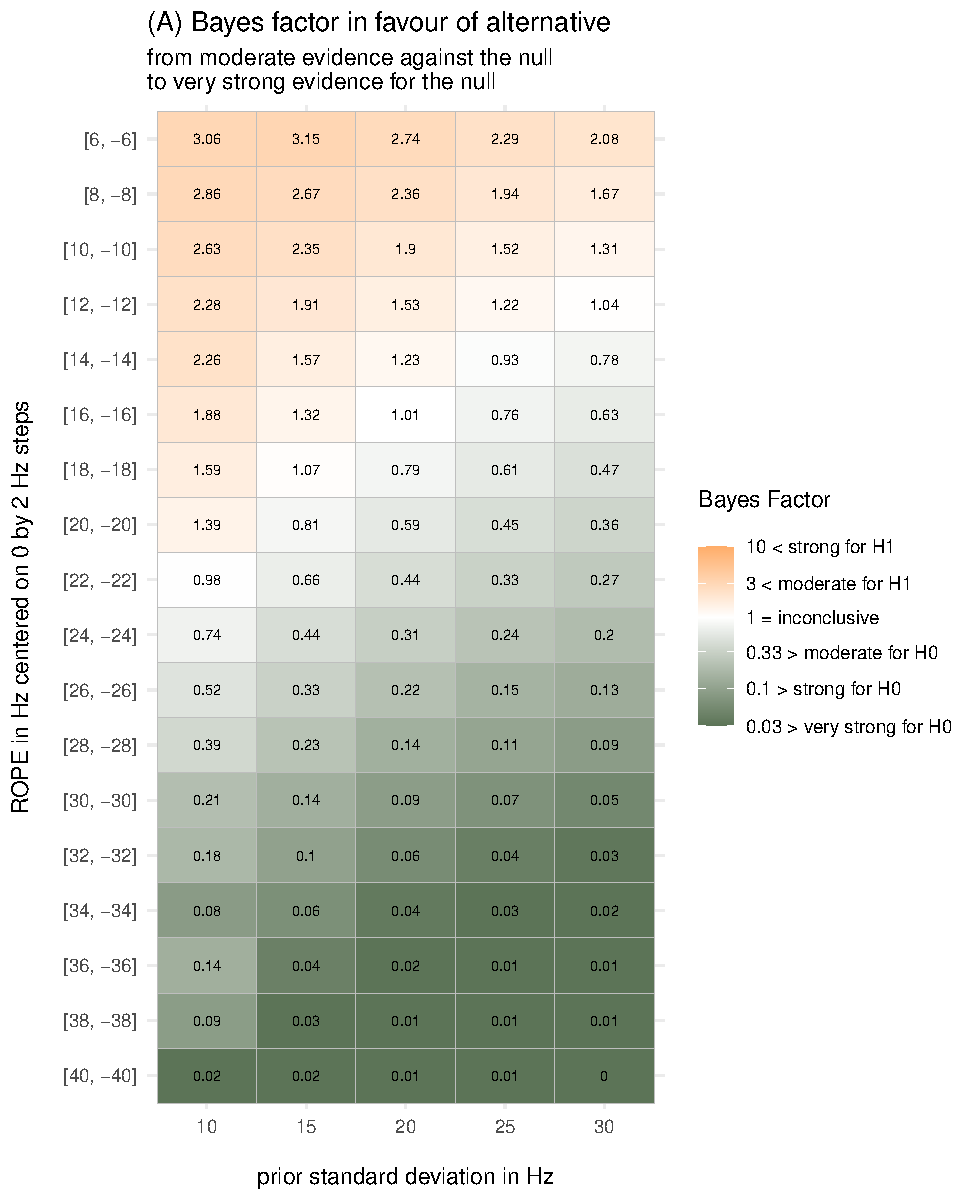
\includegraphics{manuscript_files/figure-pdf/visualize-raster-1.pdf}

}

\end{figure}%

The matrix of BFs is visualized in Figure X. Orange cells indicate
evidence for the alternative. Green cells indicate evidence for the
null. Given that you can see that the conclusions we can draw from our
data are rather dependent on the choices we made along the way.

By comparing the BF values along the y-axis, we can see that the
calculated BFs are heavily dependent on the chosen ROPE. We here chose
(theoretically speaking) a quite large range of ROPEs. The smallest ROPE
we tested (-0.05 to 0.05) corresponds to evidence that listeners can
hear pitch differences of 5\%
(\citeproc{ref-isacenko-schadlich_Model_book_1970}{Isačenko \&
Schädlich, 1970}). But even the largest ROPE we tested (-2 to 2) is
theoretically not unthinkable. 't Hart
(\citeproc{ref-thart_Differential_journalarticle_1981}{1981}) reports on
experimental evidence suggesting that listeners cannot reliably hear
pitch changes below 1.5-2 semitones. In light of this range of possible
definitions what constitutes meaningful differences, our data seem not
very robust, as illustrated by the shift from orange to green.

Additionally, when comparing the BF values along the x-axis, we can see
that the calculated BFs are comparatively robust for different standard
deviations of the critical prior. However, we can also see that the BF
values decrease with the width of the priors (from left to right). This
is not surprising and a known phenomenon, often discussed under the
Jeffreys-Lindley paradox
(\citeproc{ref-lindley_Statistical_journalarticle_1957}{Lindley, 1957}):
The more diffuse the priors are (i.e.~wider priors), the larger is the
probability that a specific parameter values is not compatible with the
data.

Combined, we can see that the larger the ROPE and the wider the priors,
the weaker the evidence for the alternative / stronger the evidence for
the null hypothesis. In an ideal world, the evidence provided by the
data should be robust across these subjective choices. But BF
calculations like these allow us to assess the boundaries of our
conclusions.

\subsection{BF for point hypothesis}\label{bf-for-point-hypothesis}

don't lol

\section{How to write things up}\label{how-to-write-things-up}

Do's Do think think about sensible priors think about sensible ropes
think about the smallest effect sizes of interest instead of testing
point-0

Don'ts Don't fall into the trap of discrete thresholds. Don't hack ropes

\section{Other Resources}\label{other-resources}

\subsubsection{References}\label{references}

\begin{verbatim}
R version 4.4.3 (2025-02-28)
Platform: x86_64-apple-darwin20
Running under: macOS Sequoia 15.5

Matrix products: default
BLAS:   /Library/Frameworks/R.framework/Versions/4.4-x86_64/Resources/lib/libRblas.0.dylib 
LAPACK: /Library/Frameworks/R.framework/Versions/4.4-x86_64/Resources/lib/libRlapack.dylib;  LAPACK version 3.12.0

locale:
[1] en_US.UTF-8/en_US.UTF-8/en_US.UTF-8/C/en_US.UTF-8/en_US.UTF-8

time zone: Europe/Oslo
tzcode source: internal

attached base packages:
[1] stats     graphics  grDevices utils     datasets  methods   base     

other attached packages:
 [1] ggdist_3.3.2        rstan_2.32.6        StanHeaders_2.32.10
 [4] see_0.11.0          bayestestR_0.16.1.2 tidybayes_3.0.6    
 [7] brms_2.22.0         Rcpp_1.1.0          ggridges_0.5.6     
[10] lubridate_1.9.4     forcats_1.0.0       stringr_1.5.1      
[13] dplyr_1.1.4         purrr_1.1.0         readr_2.1.5        
[16] tidyr_1.3.1         tibble_3.3.0        ggplot2_3.5.1      
[19] tidyverse_2.0.0    

loaded via a namespace (and not attached):
 [1] svUnit_1.0.6         tidyselect_1.2.1     farver_2.1.2        
 [4] loo_2.8.0            fastmap_1.2.0        tensorA_0.36.2.1    
 [7] digest_0.6.36        timechange_0.3.0     lifecycle_1.0.4     
[10] processx_3.8.4       magrittr_2.0.3       posterior_1.6.0     
[13] compiler_4.4.3       rlang_1.1.6          tools_4.4.3         
[16] utf8_1.2.6           yaml_2.3.10          data.table_1.17.8   
[19] knitr_1.48           labeling_0.4.3       bridgesampling_1.1-2
[22] bit_4.6.0            pkgbuild_1.4.4       cmdstanr_0.8.1      
[25] abind_1.4-5          withr_3.0.2          datawizard_1.2.0    
[28] grid_4.4.3           stats4_4.4.3         colorspace_2.1-1    
[31] inline_0.3.19        scales_1.3.0         insight_1.3.1.14    
[34] cli_3.6.5            mvtnorm_1.3-1        rmarkdown_2.27      
[37] crayon_1.5.3         generics_0.1.4       RcppParallel_5.1.8  
[40] rstudioapi_0.16.0    tzdb_0.5.0           bayesplot_1.11.1    
[43] parallel_4.4.3       matrixStats_1.3.0    vctrs_0.6.5         
[46] Matrix_1.7-2         jsonlite_2.0.0       hms_1.1.3           
[49] arrayhelpers_1.1-0   bit64_4.6.0-1        logspline_2.1.22    
[52] glue_1.8.0           codetools_0.2-20     ps_1.7.7            
[55] distributional_0.4.0 stringi_1.8.7        gtable_0.3.6        
[58] QuickJSR_1.3.0       munsell_0.5.1        pillar_1.11.0       
[61] htmltools_0.5.8.1    Brobdingnag_1.2-9    R6_2.6.1            
[64] vroom_1.6.5          evaluate_0.24.0      lattice_0.22-6      
[67] backports_1.5.0      rstantools_2.4.0     coda_0.19-4.1       
[70] gridExtra_2.3        nlme_3.1-167         checkmate_2.3.1     
[73] xfun_0.45            pkgconfig_2.0.3     
\end{verbatim}

\begin{verbatim}
[[1]]
Bürkner P (2017). "brms: An R Package for Bayesian Multilevel Models
Using Stan." _Journal of Statistical Software_, *80*(1), 1-28.
doi:10.18637/jss.v080.i01 <https://doi.org/10.18637/jss.v080.i01>.

Bürkner P (2018). "Advanced Bayesian Multilevel Modeling with the R
Package brms." _The R Journal_, *10*(1), 395-411.
doi:10.32614/RJ-2018-017 <https://doi.org/10.32614/RJ-2018-017>.

Bürkner P (2021). "Bayesian Item Response Modeling in R with brms and
Stan." _Journal of Statistical Software_, *100*(5), 1-54.
doi:10.18637/jss.v100.i05 <https://doi.org/10.18637/jss.v100.i05>.

[[2]]
Makowski D, Ben-Shachar M, Lüdecke D (2019). "bayestestR: Describing
Effects and their Uncertainty, Existence and Significance within the
Bayesian Framework." _Journal of Open Source Software_, *4*(40), 1541.
doi:10.21105/joss.01541 <https://doi.org/10.21105/joss.01541>,
<https://joss.theoj.org/papers/10.21105/joss.01541>.

[[3]]
Kay M (2023). _tidybayes: Tidy Data and Geoms for Bayesian Models_.
doi:10.5281/zenodo.1308151 <https://doi.org/10.5281/zenodo.1308151>, R
package version 3.0.6, <http://mjskay.github.io/tidybayes/>.

[[4]]
Wickham H, Averick M, Bryan J, Chang W, McGowan LD, François R,
Grolemund G, Hayes A, Henry L, Hester J, Kuhn M, Pedersen TL, Miller E,
Bache SM, Müller K, Ooms J, Robinson D, Seidel DP, Spinu V, Takahashi
K, Vaughan D, Wilke C, Woo K, Yutani H (2019). "Welcome to the
tidyverse." _Journal of Open Source Software_, *4*(43), 1686.
doi:10.21105/joss.01686 <https://doi.org/10.21105/joss.01686>.

[[5]]
Kay M (2024). "ggdist: Visualizations of Distributions and Uncertainty
in the Grammar of Graphics." _IEEE Transactions on Visualization and
Computer Graphics_, *30*(1), 414-424. doi:10.1109/TVCG.2023.3327195
<https://doi.org/10.1109/TVCG.2023.3327195>.

Kay M (2024). _ggdist: Visualizations of Distributions and
Uncertainty_. doi:10.5281/zenodo.3879620
<https://doi.org/10.5281/zenodo.3879620>, R package version 3.3.2,
<https://mjskay.github.io/ggdist/>.
\end{verbatim}

\phantomsection\label{refs}
\begin{CSLReferences}{1}{0}
\bibitem[\citeproctext]{ref-franke-roettger_Bayesian_preprint_2019}
Franke, M., \& Roettger, T. (2019). \emph{Bayesian regression modeling
(for factorial designs): {A} tutorial}. OSF.
\url{https://doi.org/10.31234/osf.io/cdxv3}

\bibitem[\citeproctext]{ref-gelman-etal_Prior_journalarticle_2017}
Gelman, A., Simpson, D., \& Betancourt, M. (2017). The {Prior Can Often
Only Be Understood} in the {Context} of the {Likelihood}.
\emph{Entropy}, \emph{19}(10), 555.
\url{https://doi.org/10.3390/e19100555}

\bibitem[\citeproctext]{ref-isacenko-schadlich_Model_book_1970}
Isačenko, A., \& Schädlich, H.-J. (1970). \emph{A model of standard
{German} intonation}. Walter de Gruyter GmbH \& Co KG.

\bibitem[\citeproctext]{ref-kruschke_Rejecting_journalarticle_2018}
Kruschke, J. K. (2018). Rejecting or {Accepting Parameter Values} in
{Bayesian Estimation}. \emph{Advances in Methods and Practices in
Psychological Science}, \emph{1}(2), 270--280.
\url{https://doi.org/10.1177/2515245918771304}

\bibitem[\citeproctext]{ref-lee-wagenmakers_Bayesian_book_2014}
Lee, M. D., \& Wagenmakers, E.-J. (2014). \emph{Bayesian {Cognitive
Modeling}: {A Practical Course}}. Cambridge University Press.

\bibitem[\citeproctext]{ref-lindley_Statistical_journalarticle_1957}
Lindley, D. V. (1957). A {Statistical Paradox}. \emph{Biometrika},
\emph{44}(1/2), 187--192. \url{https://doi.org/10.2307/2333251}

\bibitem[\citeproctext]{ref-thart_Differential_journalarticle_1981}
't Hart, J. (1981). Differential sensitivity to pitch distance,
particularly in speech. \emph{The Journal of the Acoustical Society of
America}, \emph{69}(3), 811--821. \url{https://doi.org/10.1121/1.385592}

\bibitem[\citeproctext]{ref-winter_Linear_preprint_2013}
Winter, B. (2013). \emph{Linear models and linear mixed effects models
in {R} with linguistic applications} (arXiv:1308.5499). arXiv.
\url{https://doi.org/10.48550/arXiv.1308.5499}

\bibitem[\citeproctext]{ref-winter-grawunder_Phonetic_journalarticle_2012}
Winter, B., \& Grawunder, S. (2012). The phonetic profile of {Korean}
formal and informal speech registers. \emph{Journal of Phonetics},
\emph{40}(6), 808--815. \url{https://doi.org/10.1016/j.wocn.2012.08.006}

\end{CSLReferences}






\end{document}
